\documentclass{article}
\usepackage{graphicx}
\usepackage{subfigure}
\usepackage{placeins}
\usepackage{hyperref}
\hypersetup{
    colorlinks,
    citecolor=blue,
    filecolor=blue,
    linkcolor=blue,
    urlcolor=blue
}
\newcommand{\graph}[1]{\subfigure[#1.tex]{\includegraphics[scale=0.21]{#1}}}
\begin{document}
\title{Feynman Diagrams}
\author{ATLAS SUSY Group}
\maketitle
\tableofcontents

\section*{SUSY Template}

\begin{figure}[!ht]
\centering
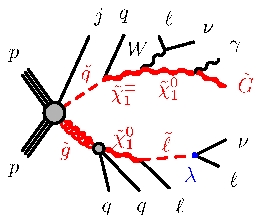
\includegraphics[width=0.5\textwidth]{ATLAS-SUSY.pdf}
\caption{ATLAS-SUSY.tex}
\end{figure}

\clearpage
\section{Interactions}

\begin{figure}[!ht]
\centering
\graph{WWZ}
\graph{CWN}
\graph{llZ}
\graph{sllN}
\graph{tbW}
\graph{stbC}
\caption{}
\end{figure}

\clearpage
%%%%%%%%%%%%%%%%%%%%%%%%%%%%%
\section{Squark and Gluino Production}

\begin{figure}[!ht]
\centering
\graph{sqsq}
\graph{sudscsudsc}
\graph{gogo}
\graph{sqgo}
\caption{}
\end{figure}

\begin{figure}[!ht]
\centering
\graph{sqsq-qqN1N1}
\graph{gogo-qqqqN1N1}
\graph{sqsq-phqqN1N1}
\graph{sqsq-jqqN1N1}
\graph{scsc-ccN1N1}
\graph{gogo-ccccN1N1}
\caption{}
\end{figure}

\begin{figure}[!ht]
\centering
\graph{sqsq-qqWWN1N1}
\graph{gogo-qqqqWWN1N1}
\graph{sqsq-qqZZN1N1}
\graph{sqsq-qqZZN1N1-hh}
\caption{}
\end{figure}

\begin{figure}[!ht]
\centering
\graph{gogo-qqqqZZN1N1}
\graph{gogo-bbbbZZN1N1}
\graph{sqsq-qqWZN1N1-h}
\graph{gogo-qqqqWZN1N1-h}
\caption{}
\end{figure}

\begin{figure}[!ht]
\centering
\graph{sqsq-qqWWZZN1N1-C1N2}
\graph{gogo-qqqqWWZZN1N1-C1N2}
\graph{gogo-qqqqWWZZN1N1-C1N2_noIndex}
\graph{sqsq-qqWWZZN1N1-C2N2}
\graph{gogo-qqqqWWZZN1N1-C2N2}
\graph{sqsq-qqlllvN1N1-C1N2}
\graph{gogo-qqqqlllvN1N1-C1N2}
\caption{}
\end{figure}

\begin{figure}[!ht]
\centering
\graph{gogo-ttttN1N1}
\graph{gogo-WWWWbbbbN1N1}
\graph{gogo-tbfftbffN1N1}
\graph{gogo-bbWffbbWffN1N1}
\graph{gogo-ttttN1N1-stst}
\graph{gogo-bbbbN1N1-sbsb}
\caption{}
\end{figure}

\begin{figure}[!ht]
\centering
\graph{gogo-tctcN1N1-stst}
\graph{gogo-tsofttsoftN1N1-stst}
\graph{gogo-tttbWZN1N1}
\graph{gogo-bbbbN1N1}
\graph{gogo-q3q3q3q3N1N1}
\graph{sqgo-qqqN1N1}
\caption{}
\end{figure}

\begin{figure}[!ht]
\centering
\graph{gogo-ttbbN1N1}
\graph{gogo-ttbbN1N1-stsb}
\graph{gogo-bbtbffN1N1}
\graph{gogo-tttbffN1N1}
\caption{}
\end{figure}

\begin{figure}[!ht]
\centering
\graph{gogo-tttthhN1N1}
\graph{gogo-ttbbhhN1N1}
\graph{gogo-bbbbhhN1N1}
\caption{}
\end{figure}

\clearpage
%%%%%%%%%%%%%%%%%%%%%%%%%%%%%
\section{Third Generation}

\begin{figure}[!ht]
\centering
\graph{stst}
\graph{sbsb}
\caption{}
\end{figure}

\begin{figure}[!ht]
\centering
\graph{stst-ttN1N1}
\graph{stst-bbWWN1N1}
\graph{stst-bqqbqqN1N1-tt}
\graph{stst-blvbqqN1N1-tt}
\graph{stst-blvblvN1N1-tt}
\caption{}
\end{figure}

\begin{figure}[!ht]
\centering
\graph{stst-bqqbqqN1N1-3body}
\graph{stst-blvbqqN1N1-3body}
\graph{stst-blvblvN1N1-3body}
\graph{stst-bqqbqqN1N1-4body}
\graph{stst-blvbqqN1N1-4body}
\graph{stst-blvblvN1N1-4body}
\caption{}
\end{figure}

\begin{figure}[!ht]
\centering
\graph{stst-bffbffN1N1-4body}
\graph{st2st2-ZZttN1N1}
\graph{st2st2-ZhttN1N1}
\graph{st2st2-ttN1N1}
\caption{}
\end{figure}

\begin{figure}[!ht]
\centering
\graph{stst-ccN1N1}
\graph{stst-ccN1N1-bWC1loop}
\graph{stst-ccN1N1-bWC1loop-ISR}
\graph{stst-ccN1N1-effective}
\caption{}
\end{figure}

\begin{figure}[!ht]
\centering
\graph{sq3sq3-q3q3N1N1}
\graph{sq3sq3-q3q3WWN1N1}
\graph{sbsb-ttWWN1N1}
\graph{sbsb-bbN1N1}
\graph{sbsb-bbN2N2}
\graph{sbsb-bbhhN1N1}
\caption{}
\end{figure}

\clearpage
%%%%%%%%%%%%%%%%%%%%%%%%%%%%%
\section{Electroweak Production}

\begin{figure}[!ht]
\centering
\graph{slsl}
\graph{staustau}
\graph{slsl-llN1N1}
\graph{staustau-tautauN1N1}
\caption{}
\end{figure}

\begin{figure}[!ht]
\centering
\graph{C1C1}
\graph{C1N1}
\graph{C1N2}
\graph{N1N1}
\graph{N2N3}
\caption{}
\end{figure}

\begin{figure}[!ht]
\centering
\graph{C1N2-WZN1N1}
\graph{C1N2-WhN1N1}
\graph{C1N23-WZN1N1}
\graph{C1N23-WhN1N1}
\caption{}
\end{figure}

\begin{figure}[!ht]
\centering
\graph{C1C1-llvvN1N1-slsl}
\graph{C1C1-llvvN1N1-slsnu}
\graph{C1C1-tautauvvN1N1-staustau}
\graph{C1C1-tautauvvN1N1-stausnu}
\caption{}
\end{figure}

\begin{figure}[!ht]
\centering
\graph{C1C1-llvvN1N1-WW}
\graph{C1C1-lvqqN1N1-WW}
\graph{Zh-llN1N1}
\graph{C1C1-jjllvvN1N1-slsl}
\graph{C1C1-jjllvvN1N1-slslSS}
\graph{C1C1-jllvvN1N1-slsl}
\graph{C1C1-jjllvvN1N1-VBFslslSS}
\caption{}
\end{figure}

\begin{figure}[!ht]
\centering
\graph{C1N2-lllvN1N1-slsl}
\graph{C1N2-lllvN1N1-slsnu}
\graph{C1N2-tautautauvN1N1-staustau}
\graph{C1N2-tautautauvN1N1-stausnu}
\graph{C1N2-jjlllvN1N1-slsl}
\caption{}
\end{figure}

\begin{figure}[!ht]
\centering
\graph{C1N2-llqqN1N1-WZ}
\graph{C1N2-lllvN1N1-WZ}
\graph{C1N2-lllvN1N1g-WZ}
\graph{C1N2-llqqN1N1g-WZ}
\graph{C1N2-lvbbN1N1-Wh}
\graph{C1N2-qqbbN1N1-Wh}
\caption{}
\end{figure}

\begin{figure}[!ht]
\centering
\graph{C1N2-lllvN1N1-Wh}
\graph{C1N2-lvqqlvN1N1-Wh}
\graph{C1N2-tautaulvN1N1-Wh}
\graph{C1N2-qqllN1N1-Wh}
\graph{C1N2-qqtautauN1N1-Wh}
\graph{C1N2-phphlvN1N1-Wh}
\caption{}
\end{figure}

\begin{figure}[!ht]
\centering
\graph{N2N3-llllN1N1-slsl}
\graph{N2N3-llllN1N1g-slsl}
\graph{N2N3-tautautautauN1N1-staustau}
\graph{N2N3-llllN1N1-ZZ}
\caption{}
\end{figure}

\begin{figure}[!ht]
\centering
\graph{C1C1-tbtbN1N1-H+H+}
\graph{C1C1-tautauvvN1N1-H+H+}
\graph{C1N2-tbbbN1N1-H+A}
\graph{C1N2-tauvtautauN1N1-H+A}
\graph{C1N2-H+N1AN1}
\caption{}
\end{figure}

\clearpage
%%%%%%%%%%%%%%%%%%%%%%%%%%%%%
\section{GGM}

\begin{figure}[!ht]
\centering
\graph{gogo-qqgtautautauvGG-GMSB}
\graph{gogo-qqqqtautautauvGG-GMSB}
\graph{gogo-qqqqphphGG-GMSB}
\graph{gogo-qqqqphZGG-GMSB}
\graph{gogo-qqqqZZGG-GMSB}
\graph{gogo-qqqqhphGG-GMSB}
\caption{}
\end{figure}

\begin{figure}[!ht]
\centering
\graph{gogo-qqqqllllGG-ZZ}
\graph{gogo-qqqqbbphGG-h}
\graph{stst-bWthZGG-GMSB}
\graph{stst-bnubnutautauGG}
\graph{hjj-phGGjj}
\graph{hjj-phphGGjj}
\caption{}
\end{figure}

\begin{figure}[!ht]
\centering
\graph{C1N1-WllllGG-ZZ}
\graph{C1N1-phlvGG-W}
\graph{C1N1-WphbbGG-h}
\graph{C1C1-WWphphGG-GGM}
\graph{N1N1-hhGG-ZZ}
\graph{N1N1-hhGG-bbbb}
\graph{slsl-llGG-GMSB}
\caption{}
\end{figure}

\clearpage
%%%%%%%%%%%%%%%%%%%%%%%%%%%%%
\section{RPV and Long-Lived Decays}

\subsection{AMSB} 

\begin{figure}[!ht]
\centering
\graph{C1C1-gpipiN1N1-AMSB}
\graph{C1N1-gpiN1N1-AMSB}
\graph{C1C1-qpipiN1N1-AMSB}
\graph{C1N1-qpiN1N1-AMSB}
\graph{C1C1-jpipiN1N1-AMSB}
\graph{C1N1-jpiN1N1-AMSB}
\caption{}
\end{figure}
\clearpage

%%%%%%%%%%%%%%%%%%%%%%%%%%%%%
\subsection{Disappearing track search}

\begin{figure}[!ht]
\centering
\graph{gogo-qqqqpipiN1N1}
\caption{}
\end{figure}

\clearpage
\subsection{LLE Operator ($\lambda$)}

\begin{figure}[!ht]
\centering
\graph{N1emv-slL}
\graph{N1emv-slR}
\graph{N1emv-snu}
\graph{N1etv-slL}
\graph{N1etv-slR}
\graph{N1etv-snu}
\caption{}
\end{figure}

\begin{figure}[!ht]
\centering
\graph{N1N1-llvllv-slsl-RPV}
\graph{N1N1-llvllv-snusnu-RPV}
\graph{gogo-qqqqllllvv-RPV}
\graph{C1C1-WWllllvv-RPV}
\graph{slsl-llllllvv-RPV}
\graph{svsv-llllvvvv-RPV}
\caption{}
\end{figure}

\begin{figure}[!ht]
\centering
\graph{WH-N1N1-4l2nu-RPV}
\graph{ZH-N1N1-4l2nu-RPV}
\caption{}
\end{figure}

\begin{figure}[!ht]
\centering
\graph{stst-ttmumutautauvv-RPV}\\
\caption{}
\end{figure}

\clearpage
\subsection{LQD Operator ($\lambda^{\prime}$)}

\begin{figure}[!ht]
\centering
\graph{sqsq-qqlqql-N1N1-RPV}
\graph{sqsq-2q2nu4l-N1N1-RPV}
\graph{sneut-ll-RPV}
\graph{sneut-emu-RPV}
\graph{sneut-etau-RPV}
\graph{sneut-mutau-RPV}
\caption{}
\end{figure}

\clearpage
\subsection{UDD Operator ($\lambda^{\prime\prime}$)}

\begin{figure}[!ht]
\centering
\graph{sqsq-4q4q-RPV}
\graph{gogo-3q3q-RPV}
\graph{gogo-5q5q-RPV}
\graph{gogo-4t-6q-RPV}
\graph{gogo-ttqqqq-stst-RPV}
\graph{gogo-ttbbss-stst-RPV}
\caption{}
\end{figure}

\begin{figure}[!ht]
\centering
\graph{stst-qqqq-RPV}
\graph{stst-bsbs-RPV}
\graph{WH-N1N1-6q-RPV}
\graph{ZH-N1N1-6q-RPV}
\caption{}
\end{figure}

\begin{figure}[!ht]
\centering
\graph{sglsgl-gggg}\\
\caption{}
\end{figure}

\clearpage
\subsection{R-hadron searches}

\begin{figure}[!ht]
\centering
\graph{gogo-qqvsqvsq-qqqqN1N1}
\graph{go-qvsq-qqN1}
\caption{}
\end{figure}


\end{document}
